% Appendix D

% variables
\newcommand{\appdird}{appendices/plots/appendixD}

\chapter{Algorithms and particle tracking}

\label{AppendixD}


\section{Momentum reconstruction}
\label{appD:sec:mom-reco}

Momentum reconstruction is performed in two different ways in NA64. The first one consists of the analytical solution of the expected curvature of the charged particle when it enters the magnetic field. As the momentum of the primary particle is generally very high compared to its mass, this can be safely ignored. The particle travels in a straight line outside the magnets, whereas inside it the trajectory corresponds to a circle tangent to the particle entrance line. The radius of the circle is in the relativistic limit:

\begin{equation}
  \label{eq:gyro-radius}
  r_c = 3.3 \times \frac{p}{\left|q\right|B}
\end{equation}

where $\left|q\right|$=1 in most of the cases of interest. In the NA64 setup, the magnetic field is homogeneous (with deviations from the average field at $\lesssim 1\%$) and with a total length of 4 \si{\meter}. To reconstruct the momentum, a minimum of three points is required, two are needed to measure the entrance point of the particle in the magnetic field (or the exact exit point) and the third one is used to measure the exact deflection. By assuming an exact knowledge of $B$, the momentum can be reconstructed analytically. In NA64, the first two Micromegas upstream is used to measure the exact entrance point of the electron, while the 4 downstream are used to measure the deflection after its passage in the magnets. This gives a total of 4 different momentum estimates, that are used to both calculate the best momentum as the weighted average between estimates, and the goodness of the track via a $\chi^2$-test.

The approach above has the advantage of being straightforward and fast to compute but does not take into account multiple scattering experienced by the particle between Micromegas. A more sophisticated method was used for the visible mode analysis, based on the Kalman-filter implemented in the Genfit software library \cite{genfit}. A review of the method is given in Sec.\ref{appD:sec:kalman-filter}. For the final estimate, the momentum is in this case fitted globally using the information from all detectors. The design of Genfit makes it also easy to include a precise account of the material budget using a Geometry Description Markup Language (GDML) that can be extracted by the Geant4 simulation \cite{gdml}.

\subsection{Three point momentum extrapolation}
\label{appD:sec:mom-reco-simple}

The momentum reconstruction, $p_\perp^\text{reco}$, is a three-step procedure \cite{na64-muon-note}. As inputs are required a set of three hit positions $S=\{\mathbf{x}_1,\mathbf{x}_2,\mathbf{x}_3\}$ corresponding to the Micromegas MM$_1$, MM$_2$ and MM$_3$ (upstream and downstream the magnet), the dimension (length $L$ and starting and ending points) of the MBPL magnet MS2 as well as its magnetic field magnitude, $B=|\mathbf{B}|$.

In a first step, the 3-dimensional line defined by the hits upstream the magnet, $\mathbf{x}_1$ and $\mathbf{x}_2$, is extrapolated to the plane of MM$_5$ using a parametric line equation $\mathbf{p}(t)=\mathbf{p}_0+\mathbf{u}\cdot t$. The distance between $\mathbf{x}_3$ and the extrapolated point $\mathbf{x}_3^{e}$, is then extrapolated back to the magnet end ($h$). In a second step, the radius of curvature $r_c$ is calculated from geometrical considerations (see Fig. \ref{fig:momentumgeo}).
\begin{figure}[tbh!]
    \centering
    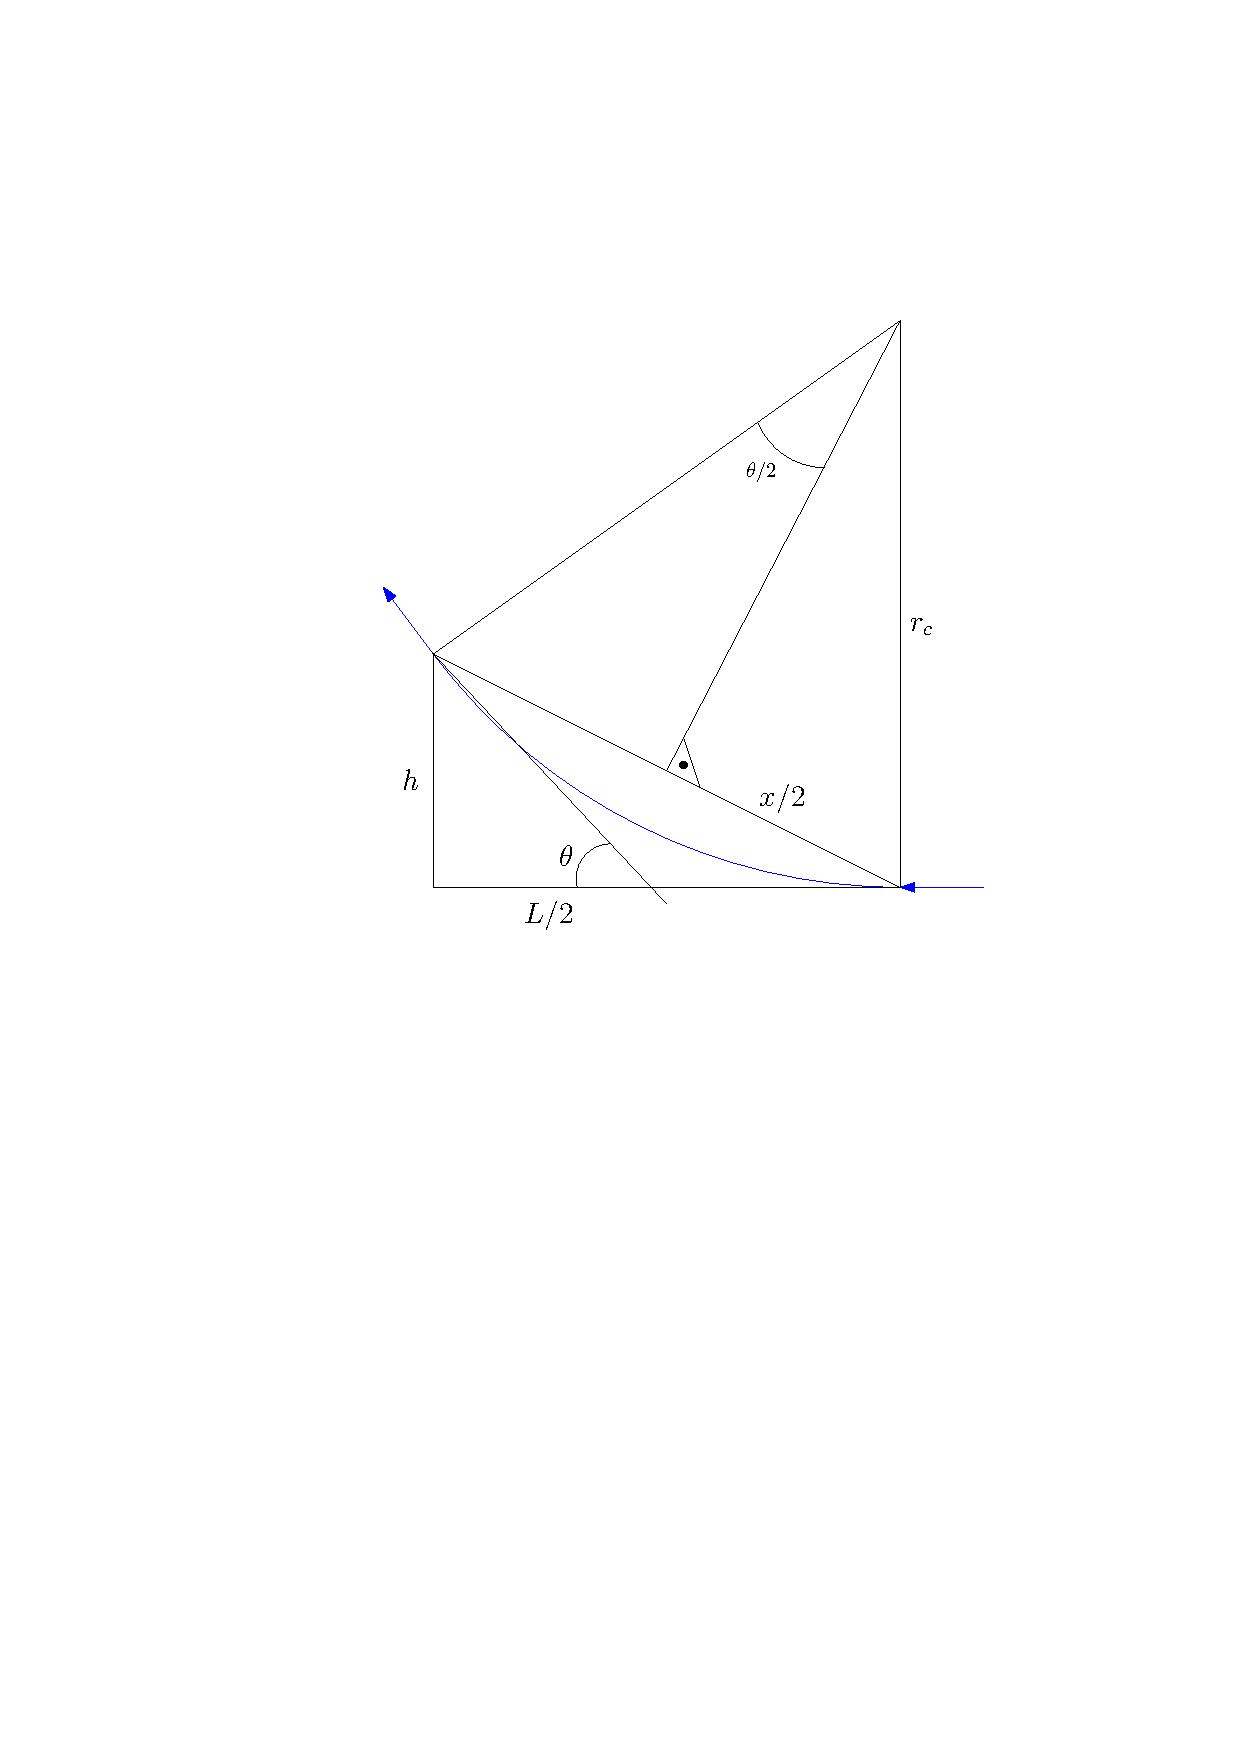
\includegraphics[width=0.5\textwidth]{\appdird/momentum.pdf}
    \caption{Two dimensional geometrical representation of a particle trajectory (blue) deflection in a uniform magnetic field.}
    \label{fig:momentumgeo}
\end{figure}
In the small angle approximation ($\sin\theta=\theta+\mathcal{O}(\theta^2)$ and $\tan\theta=\theta+\mathcal{O}(\theta^2)$), the following quantities are defined:
\begin{equation}
  \label{eq:mom-simple}
        \sin\frac{\theta}{2}\simeq\frac{x}{2r_c},\hspace{5mm}
        \tan\theta\simeq\frac{2h}{L},\hspace{5mm}x=\sqrt{h^2+L^2}=h\sqrt{1+\left(\frac{L}{h}\right)^2}\Rightarrow r_c\simeq\frac{L}{2}\sqrt{1+\left(\frac{L}{h}\right)^2}
\end{equation}
Finally the radius is projected on the beam axis and the momentum is obtained from the well-known relation $p_\perp^\text{reco}=0.3eBr_c$. 
\subsection{Genfit and the Kalman filter}
\label{appD:sec:kalman-filter}

A more sophisticated method to reconstruct track and vertices is the Kalman filter, which is widely used for track fitting and vertex reconstruction in high-energy physics \cite{HOPPNER2010518}.

The extended Kalman filter, used for the reconstruction of track and vertices, consists of a recursive algorithm to find the optimum estimate $\vec{x}_{reco}$ of the unknown true state vector $\vec{x}_{true}$. In NA64, this is implemented using the Genfit library \cite{genfit}, which seamlessly introduces the Kalman filter using objects defined in the ROOT framework \cite{root}. This greatly simplifies their manipulation in the reconstruction code. One of the main differences from the approach described in the previous section is that all error sources can be included easily in the algorithm using a noise matrix that carries the information over all possible uncertainties. This is particularly important for multiple scattering since this error depends on the amount of material between the two detectors where the particle is being propagated and is not straight forward to compute analytically, as it depends on the exact particle direction and its kinetic energy.

An initial state is required as seed for the algorithm, as the Kalman filter propagates an initial state $\vec{x}_0$ through steps $\vec{x}_k \rightarrow \vec{x}_{k+1}$ that converge asymptotically to the optimal estimate $\vec{x}_{reco}$. In NA64, the track initial state is located on the first GEM hit recorded, with a momentum in the direction of the second GEM detector hit. To compute multiple scattering corrections, the momentum can as well be relevant, as in its Gaussian approximation the Root Mean Square width is given by \cite{review-particle-physics}:

\begin{equation}
  \label{eq:mm-scattering}
  \theta_{plane}^{rms} = \frac{13.6 \mev}{\beta c p} z \sqrt{\frac{x}{X_0}} \left[ 1 + 0.038 \ln{\frac{x z^2}{X_0 \beta^2}} \right]
\end{equation}

Where $p$, $\beta c$ and $z$ are the momentum, velocity, and charge number of the incident particle, and $x/X_0$ is the thickness of the scattering medium in radiation lengths. Inside the decay volume of the visible mode, a magnetic spectrometer is not present, which means the momentum of each track is not known. To initialize the vector magnitude, the energy measured by the ECAL downstream is assumed to be equally shared between the track candidates detected in the decay volume.

Before computing a step, we define the vector $\vec{x}_k$ and the covariance matrix $C_k$ of the particle in the step $k$, which contains the information of all previous iterations. Next, we define a \textit{prediction}, where both state vector and covariance matrix are extrapolated to a state vector $\vec{x}_{k+1}^{pred}$ and $C_{k+1}^{pred}$. The covariance matrix $C_{k+1}$ is calculated by the sum of the track covariance matrix, which is in turn computed using Gaussian error propagation by the transformation of the Jacobian matrix of the propagation, and a noise matrix that takes into account the multiple scattering experienced in-between the two states. The predicted new state vector is then compared to the value measured by the tracking chamber, and corrected using this information. If we define as $\vec{x}_{k+1}^{mes}$ as the hit measured by the tracking chamber where the track is being extrapolated, this means:

\begin{equation}
  \label{eq:kf-updates}
  \begin{aligned}  
    &\underline{\vec{x}_{k+1} = \vec{x}_{k+1}^{pred} + K_{k+1} \cdot \vec{r}_{k+1}} \\
    &C_{k+1} = ( I - K_{k+1} \cdot H_{k+1} )C^{pred}_{k+1} \\
    & \\
    &\vec{r}_{k+1} = \vec{x}_{k+1}^{mes} - H_{k+1} \cdot \vec{x}_{k+1}^{pred} \\
    &K_{k+1} = C^{pred}_{k+1} H^T_{k+1}(H_{k+1}C_{k+1}^{pred}H^T_{k+1} + V_{k+1})^{-1}    
  \end{aligned}
\end{equation}

Where the matrix $K_{k+1}$ is called Kalman gain, is the covariance matrix of the measurement $\vec{x}_{k+1}^{mes}$. The projection matrix $H_{k+1}$ is a linear transformation from the coordinate system of the state vector $\vec{x}_{k+1}$ to the coordinate system of the measured state. As the elements of $C_k$ shrink after every step, the correction of the estimate becomes less relevant the more information was already processed by the algorithm. After each hit of the track was used in a Kalman step, the fit is repeated in the opposite direction, starting with $k = N_{hits}$ and performing again the process in reverse. This is done to correct for possible biases of the initial estimate $\vec{x}_0$ used as input of the algorithm. In this second round, the first fit result is used as starting value, and the covariance matrix is multiplied by a large factor ($\sim 1000$), to avoid redundancy of the information from the first fit performed.

The Genfit library reconstructs tracks using the algorithm described above and at the same time provides a framework that takes care of the exact track representation used for the fit and the hit reconstruction. Changing representation is also performed automatically for the covariance matrix and the reference plane when needed.


\begin{figure}[bth!]
  \centering
  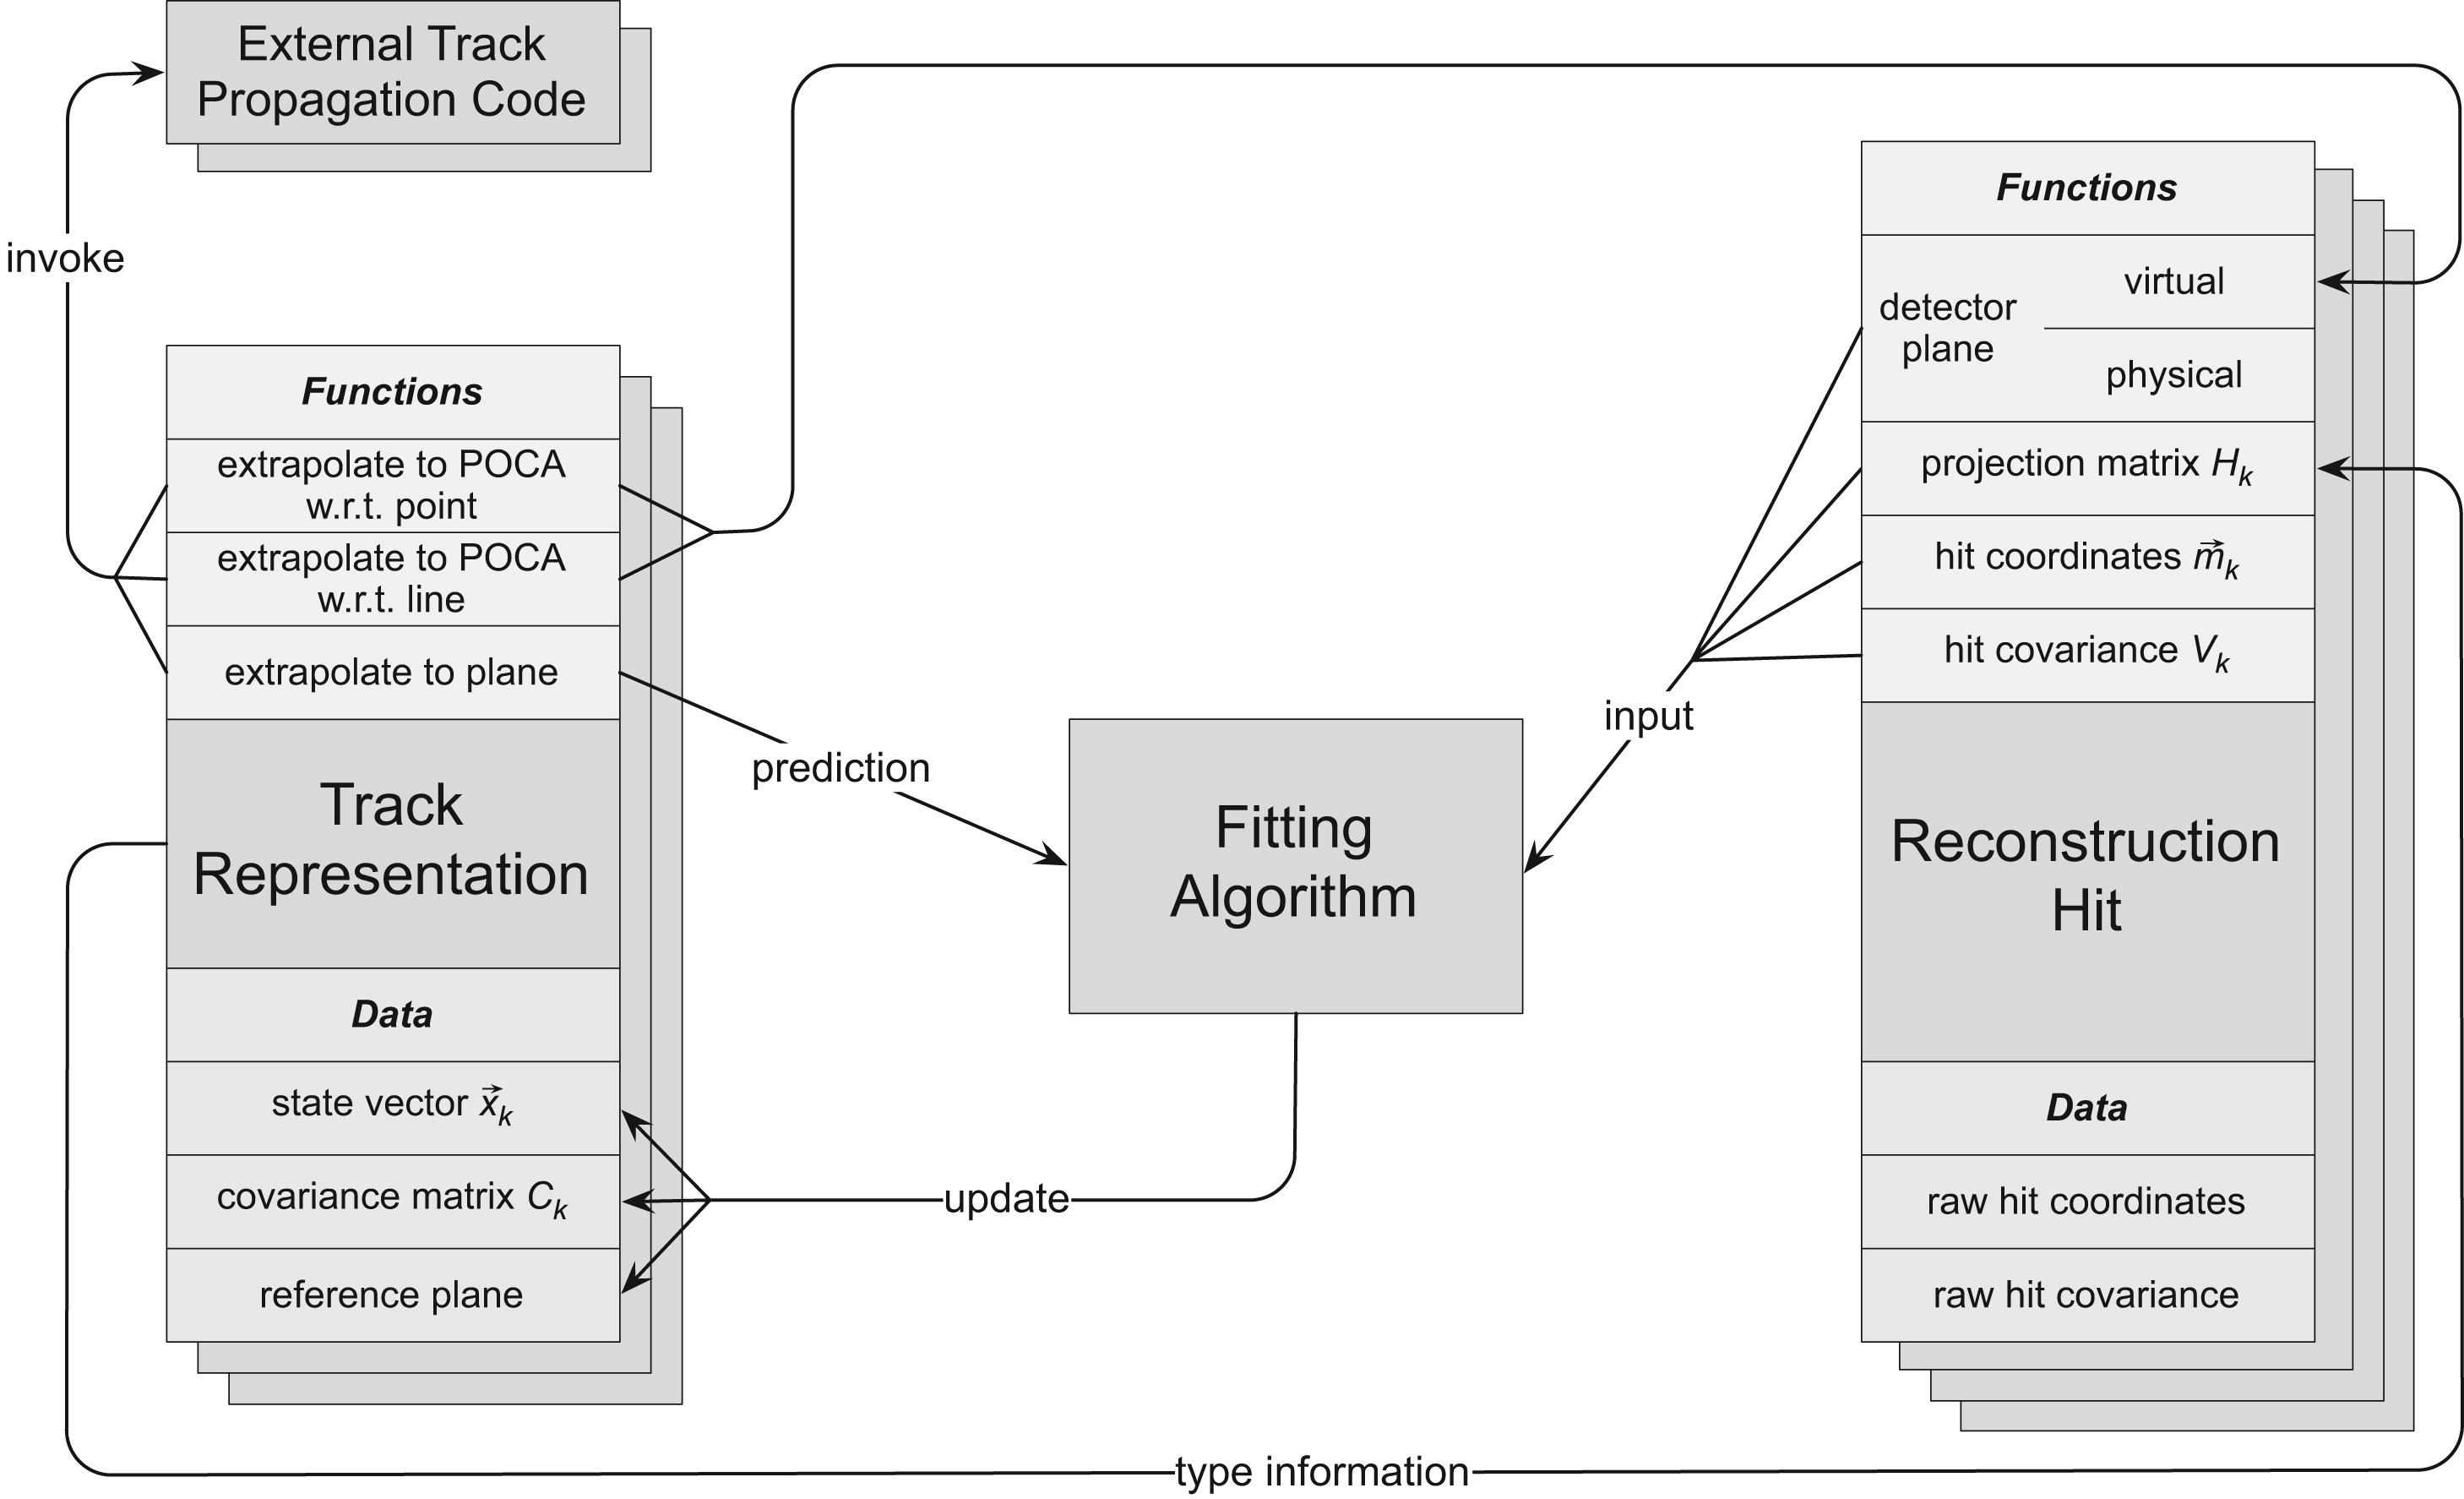
\includegraphics[width=\textwidth]{\appdird/genfit-flowchart.jpg}
  \caption[genfit flow diagram]{General structure of the objects used for track fitting. The arrow indicate the relation between objects. POCA stands for point of closest approach \cite{genfit}.}
  \label{fig:genfit-diag}
\end{figure}

To reconstruct vertices, a simple approach based on the back-propagation of the reconstructed tracks is used. The tracks reconstructed by Genfit are paired following the prescription described in Sec.\ref{ch3:sec:vis-mode-tracking}. After that, tracks are back-propagated using Genfit to the point of minimum distance in an iteration algorithm with a step length of \SI{1}{\milli\meter}. A code snippet of the function used is presented below.

\begin{lstlisting}
  double TrackProximity(genfit::Track * track1, genfit::Track * track2, TVector3 * POCA, TVector3 * mom1, TVector3 * mom2) {
    
    // Start from first measurement point
    genfit::StateOnPlane msop1 = track1->getFittedState();
    genfit::StateOnPlane msop2 = track2->getFittedState();

    TVector3 xpos1 = msop1.getPos();
    TVector3 xpos2 = msop2.getPos();
    
    // First determine which direction the tracks will get closer
    double h=0.1; //in cm
    int steps=0;
    double d = 99999999;
    double oldd=999999;
    double posd=99999;
    double negd=99999;
    oldd = (xpos1-xpos2).Mag();
    // step with positive h
    try{
      track1->getCardinalRep()->extrapolateBy(msop1,h);
      track2->getCardinalRep()->extrapolateBy(msop2,h);
    }
    catch(genfit::Exception& e){
      std::cerr << e.what();
      std::cerr << "Exception, next track" << std::endl;
    }
    xpos1 = msop1.getPos();
    xpos2 = msop2.getPos();
    posd = (xpos1-xpos2).Mag();
    // step back to original position
    try{
      track1->getCardinalRep()->extrapolateBy(msop1,-h);
      track2->getCardinalRep()->extrapolateBy(msop2,-h);
    }
    catch(genfit::Exception& e){
      std::cerr << e.what();
      std::cerr << "Exception, next track" << std::endl;
    }
    d = (xpos1-xpos2).Mag();

    // step with negative h
    try{
      track1->getCardinalRep()->extrapolateBy(msop1,-h);
      track2->getCardinalRep()->extrapolateBy(msop2,-h);
    }
    catch(genfit::Exception& e){
      std::cerr << e.what();
      std::cerr << "Exception, next track" << std::endl;
    }
    xpos1 = msop1.getPos();
    xpos2 = msop2.getPos();
    negd = (xpos1-xpos2).Mag();

    if(negd < posd){
      h = -1.0*h;
      d = negd;
    }else{
      d = posd;
    }

    while(d < oldd){
      oldd = d;
      try{
        track1->getCardinalRep()->extrapolateBy(msop1,h);
        track2->getCardinalRep()->extrapolateBy(msop2,h);
      }
      catch(genfit::Exception& e){
        std::cerr << e.what();
        std::cerr << "Exception, next track" << std::endl;
      } 
      xpos1 = msop1.getPos();
      xpos2 = msop2.getPos();
      d = (xpos1-xpos2).Mag();
      steps++;
    }

    // step back once 
    try{
      track1->getCardinalRep()->extrapolateBy(msop1,-h);
      track2->getCardinalRep()->extrapolateBy(msop2,-h);
    }
    catch(genfit::Exception& e){
      std::cerr << e.what();
      std::cerr << "Exception, next track" << std::endl;
    } 

    *mom1 = msop1.getMom();
    *mom2 = msop2.getMom();
    
    TVector3 poca = (xpos1+xpos2)*0.5;
    *POCA = poca;
    
    return d;
  } 
\end{lstlisting}


\section{Pulse reconstruction}

This section gives a brief overview of the pulse reconstruction procedure used in NA64 which translates the raw data received by the DAQ in the energy measured by a specific detector. The same procedure is applied to all detectors.

The input of this algorithm comes from the 25 16-bit samples separated by \SI{12.5}{\nano\second} each and saved by the Event Builder PC (see Fig.\ref{fig:daq}). Each sample consists of a number between 0 and 4095. The additional input of the algorithm is calculated beforehand using calibration runs: a calibration constant $K$ used to convert the raw sample into an estimate of the energy deposit and the expected arrival time $t_E$. This last value is obtained using a Gaussian fit of $t_{S_0} - t_{\rm{cell}}$ for each active cell in the setup, i.e. the reconstructed time is compared to the time recorded by the scintillator $S_0$ placed in front of the beam inlet. The sigma of the fit is also stored as the uncertainty of this value in a separate array.

Using this input the energy is reconstructed in an event in the following way:

\begin{enumerate}
\item The pedestal of the event is calculated. The first 8 samples are used for this purpose, as no interaction is expected in this time window. As the DAQ receives data from two different multiplexers\footnote{This is done to increase the rate of sampling from \SI{20}{\mega\hertz} to \SI{40}{\mega\hertz}.}, two different pedestals are defined separately for the even and odd samples. In each of these cases, it is computed as the mean ADC count between the samples in the range defined. If the difference between the largest and the smallest sample is larger than 20 ADC counts, the event is flagged as pileup, and the pedestal is set to the minimum value recorded.
\item The pedestal is subtracted to every sample of the cell. If a sample becomes negative because of this, its value is set to zero instead.
\item A peak search algorithm is run to find all peaks between sample 10 and the last one recorded. A peak is defined by a sample with a value larger than the one of its neighboring samples. All peaks are saved in a separate vector.
\item A time is extracted for each peak. The calculation is performed using the rising edge of the signal to calculate the $t_0$ of the event. The code used for the purpose is shown below.
\item A specific peak is selected as a candidate for the primary particle. Different methods were implemented and tested for this purpose. The NA64 standard is to select the peak whose $t_0$ is most compatible with the expected arrival time $t_E$. The energy is set to zero if the best peak is more than $4\sigma_t$ away from this value, where $\sigma_t$ is the uncertainty of the expected arrival time.
\item The energy of the peak selected is extracted by multiplying the calibration constant to the ADC value of the maximum peak.
\end{enumerate}

We provide two examples of this algorithm in Fig.\ref{fig:pulse-example} and Fig.\ref{fig:pulse-example-pileup}. In the first picture, we show the pulse of a common event with a single particle in the trigger. In the second, one primary activates the trigger with a second particle injected in the setup $\sim$\SI{100}{\nano\second} after.

\begin{figure}[bth!]
  \centering
  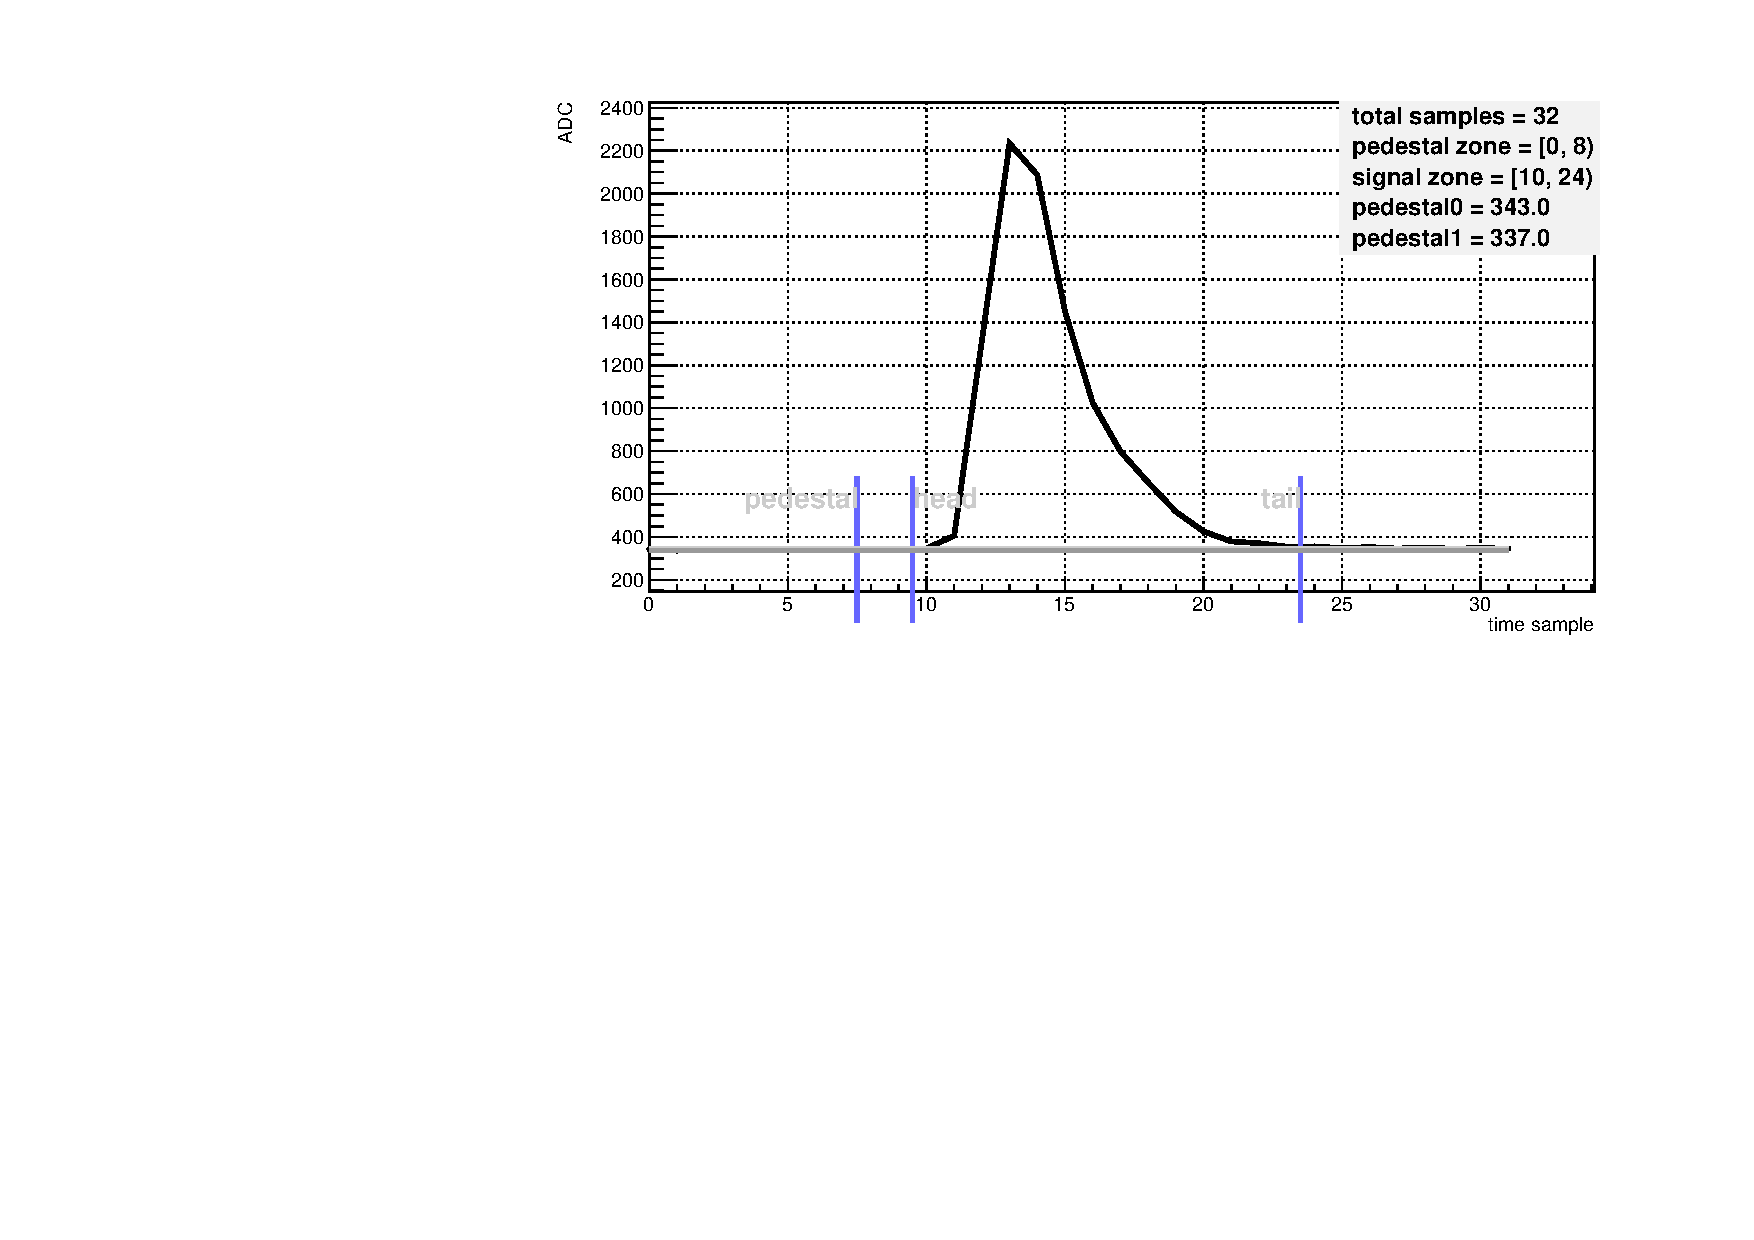
\includegraphics[width=\textwidth]{\appdird/raw-ecal33.pdf}
  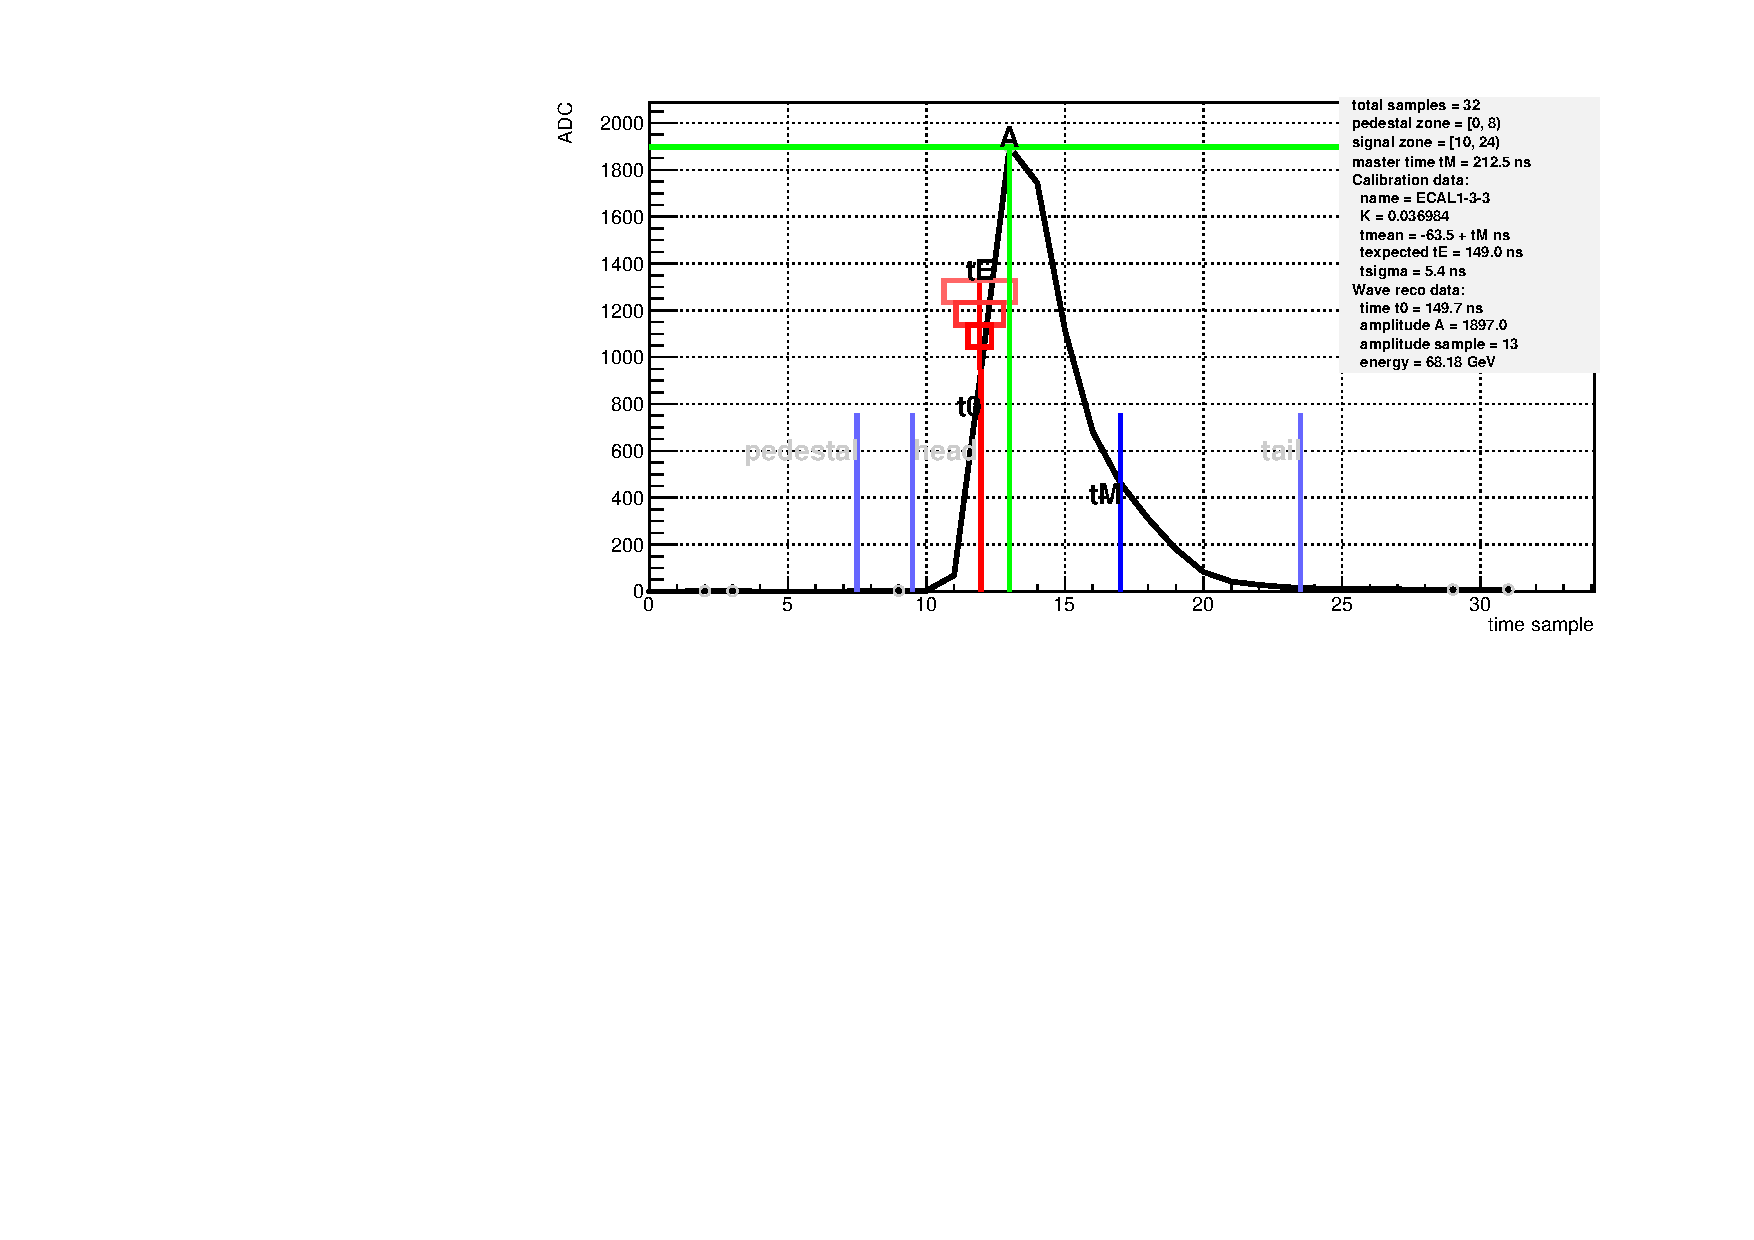
\includegraphics[width=\textwidth]{\appdird/wave-ecal33.pdf}
  \caption[example of pulse reconstruction in NA64]{Example of reconstruction of the pulse for the central cell of the ECAL for a single primary in the trigger. On the top, the pulse is shown before any treatment is applied to the waveform. On the bottom, the waveform is shown after the pedestal is subtracted and the best peak is selected. The expected time of arrival is drawn with a red line, with three squares covering an area with 1-2-3 $\sigma_t$ uncertainty respectively.}
  \label{fig:pulse-example}
\end{figure}

\begin{figure}[bth!]
  \centering
  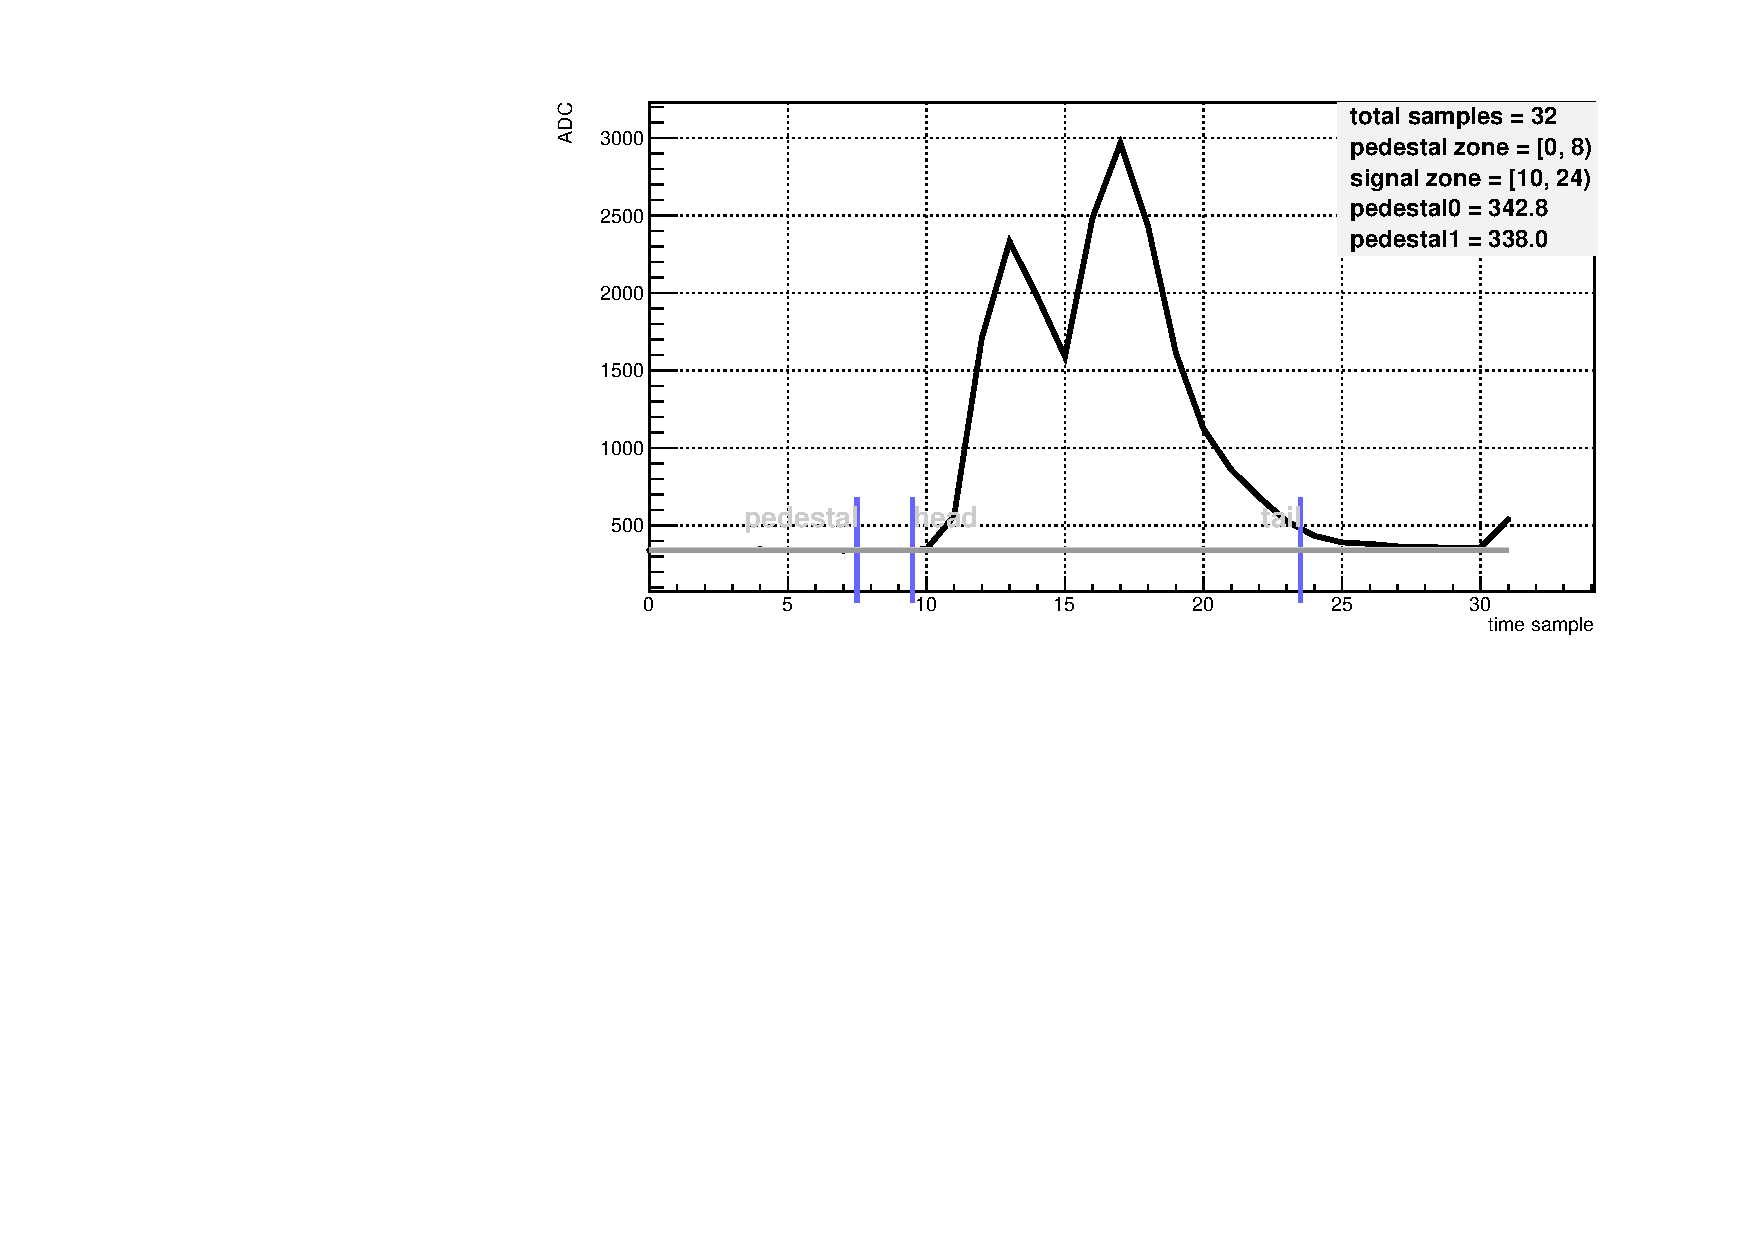
\includegraphics[width=\textwidth]{\appdird/raw-pil-ecal33.pdf}
  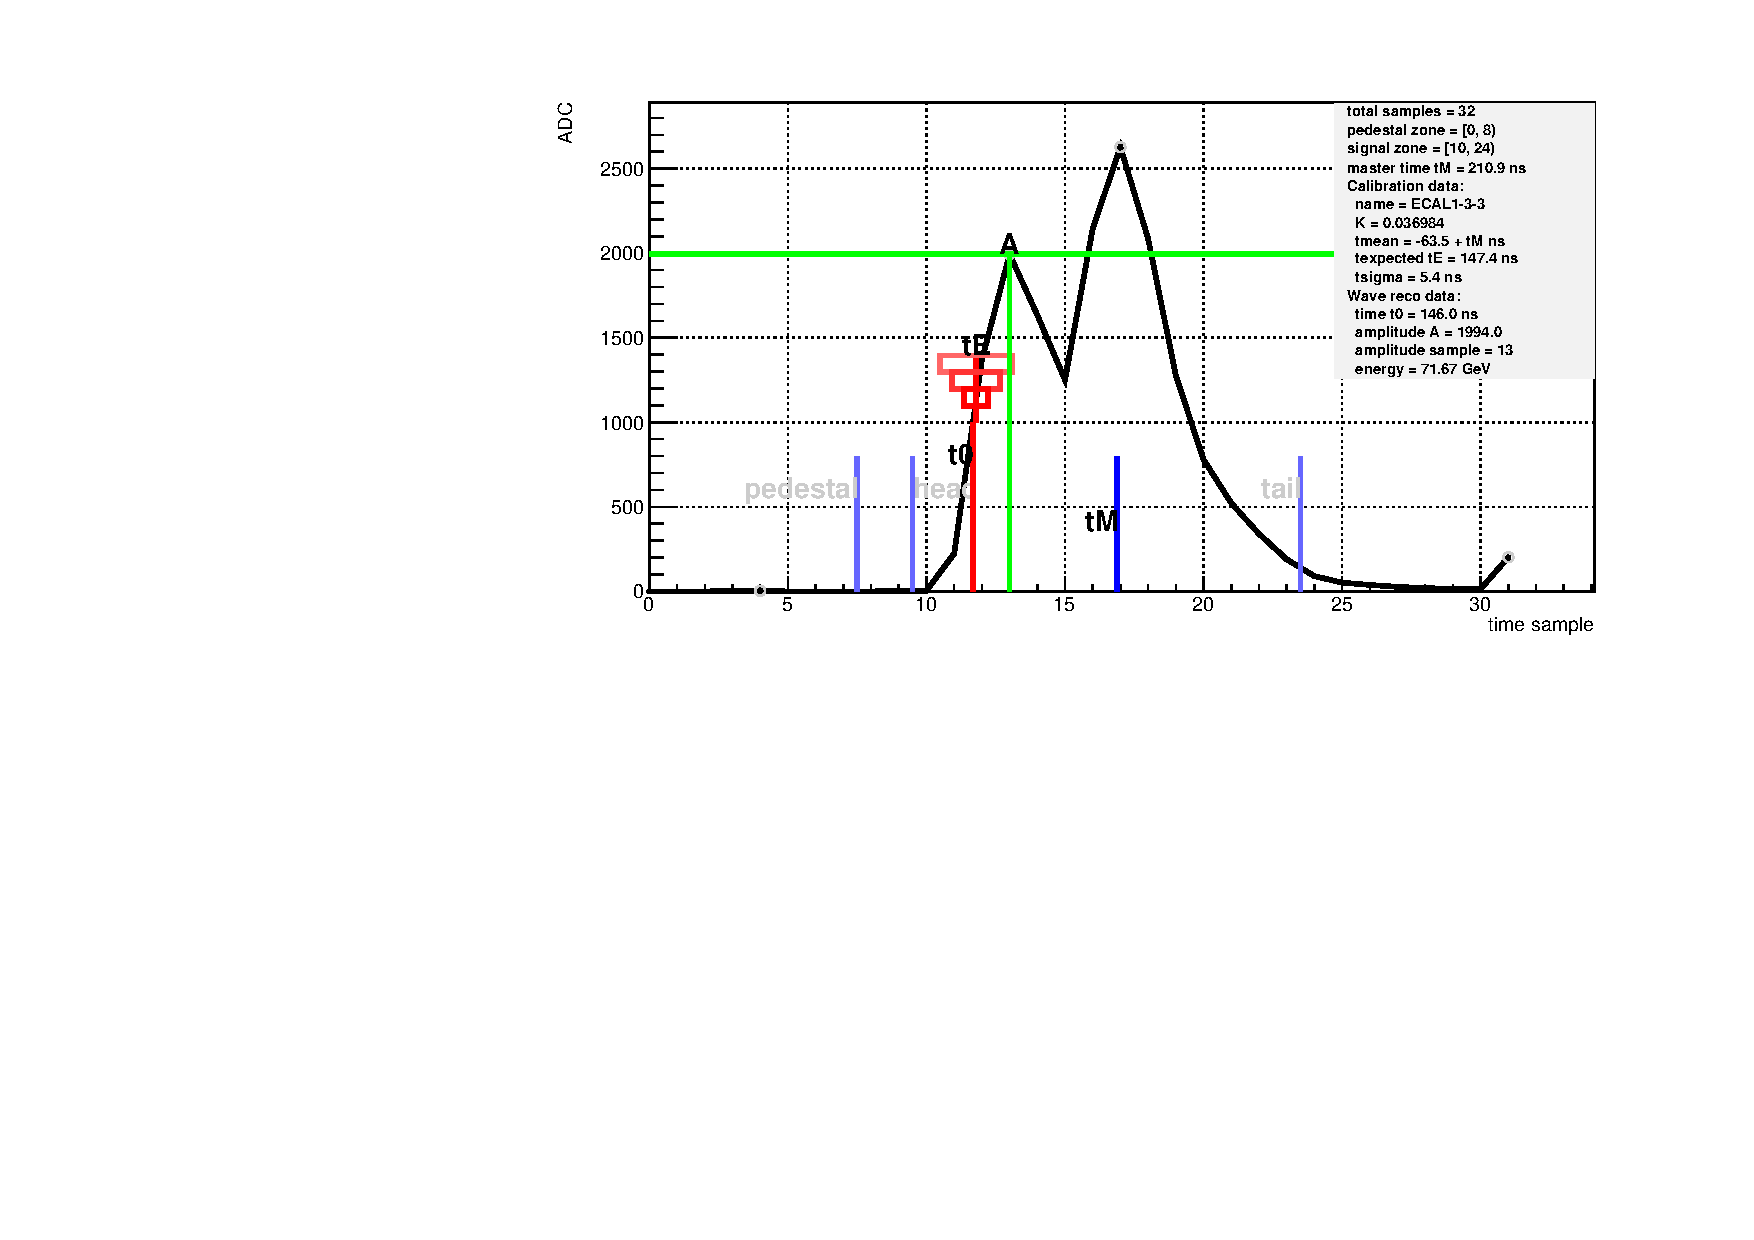
\includegraphics[width=\textwidth]{\appdird/wave-pil-ecal33.pdf}    
  \caption[example of pulse reconstruction in NA64]{Example of reconstruction of the pulse for the central cell of the ECAL for two primaries in the trigger. On the top, the pulse is shown before any treatment is applied to the waveform. On bottom, the waveform is shown after the pedestal is subtracted and the best peak is selected. The expected time of arrival is drawn with a red line, with three squares covering an area with 1-2-3 $\sigma_t$ uncertainty respectively.}
  \label{fig:pulse-example-pileup}
\end{figure}
\clearpage
\newpage
\FloatBarrier
\begin{lstlisting}
  double t0_RisingEdge(const int i_max) const
  {      
      // search for rising edge
      // https://indico.cern.ch/event/569549/contributions/2302932/
      // run the search in the backward direction from `i_max` to ensure the
      // t0 edge corresponds to `A_max` sample
      const double A_max = wave(i_max);
      const double A_half = 0.5*A_max;
      double A_min = A_max;
      const double noise = 1.;
      
      for (int i = i_max-1; i > 0; --i) {
        const double wi = wave(i);
        
        // check the rising edge is end
        if (wi > A_min + noise) break;
        if (A_min < wi) A_min = wi;
        
        // check the 0.5*A_max cross condition
        const bool cross05 = (wi <= A_half);
        if (!cross05) continue;
        
        // check the segment is rising
        const double wi1 = wave(i+1);
        const bool rising = (wi < wi1);
        if (!rising) continue;
        
        // calculate intersection of the rising edge with time axis to get origin time
        const double t0_rise = (i+1) - wi1/(wi1 - wi);
        
        if (SADC_t0_method == kT0_RisingEdgeHH) {
          const double t0_hh = t0_rise + A_half/(wi1 - wi);
          return t0_hh;
        }
        return t0_rise;
      }
      return 0.;
  }
\end{lstlisting}

%%% Local Variables:
%%% mode: latex
%%% TeX-master: "../PhDthesis"
%%% End: